\documentclass{notube}
\usepackage{capt-of}
\usepackage{url}
\makeatletter
\g@addto@macro{\UrlBreaks}{\UrlOrds}
\makeatother

\WP{7c} \WPName{Internet TV in the Social Web}

\delID{7c.4} \delName{Social TV Integrated Prototype of v.1 and v.2}
\delNameRunning{Deliverable D7c.4} \delCoordinators{Libby Miller (BBC)}

\delContributors{Vicky Buser (BBC), Dan Brickley (VU)}

\delQualityAssessor{Luca Vignaroli}

\delQualityController{Lyndon Nixon}

\dueContractual{M33}
\dueActual{31-10-11}
\status{0.9}

%\final

%\prototype
\report
%\dissemination

\public
%\consortium

\authorPartner{Libby Miller (BBC),  Vicky Buser (BBC),  Dan Brickley (VU)}
\responsibleAuthor{Libby Miller (BBC)}
\responsibleAuthorPartner{BBC}
\responsibleAuthorEmail{libby.miller@bbc.co.uk}
\responsibleAuthorPhone{+44 (787) 6565561}

\summary{
This document summarises the work done so far in the workpackage `TV and the Social web' (WP7c). It describes the approach we have taken, the prototypes we have made, and our plans for the final three months of the project.
}

\abstract{
In the workpackage `TV and the Social web' (WP7c) we have used \\
lightweight prototyping techniques in order to explore social TV in \\
on-demand, live TV, and second screen authoring environments, \\
using multi-screen environments. Our conclusions are that using \\
metadata as an advert for TV programmes, unique URLs for TV, and \\
APIs to TV and TV-like devices would make second screen applications\\
significantly more useful and interesting.
}

\keywords{TV, television, set top box, media centre, iphone, ipad, XMPP, jabber, \\
strophe, voting, companion device, second screen, authoring tools,\\ 
HTML5
}

\versionLog{
    \versionLogEntry{\today}{Libby Miller}{0.9}
}


\begin{document}

\maketitle

%\include{abbreviations}

\chapter{Introduction}

\section{Deliverable Objective}

The aim of this deliverable, D7c.4, is to:
\begin{itemize}
\item{Describe the approach we have taken throughout the project}
\item{Summarise the work we have done so far}
\item{Describe the principles behind the work}
\item{Describe the results}
\item{Describe our plans for the final months}
\end{itemize}


\section{Approach}

As defined in our first deliverable, our approach throughout the project has been to:

\begin{itemize}
\item{Enhance TV user experience by helping users find content they enjoy by making TV more social}
\end{itemize}

by

\begin{itemize}
\item{Being able to flexibly and quickly demonstrate ideas in a compelling fashion}
\item{Allowing users to share information and recommendations and create textual user generated content - essentially metadata about television - using appropriate social media tools}
\item{Enabling users to share their profile information while respecting user privacy}
\item{Testing the result with BBC content}
\end{itemize}

\noindent Two things became clear early on in this project:

\begin{itemize}
\item{Social media and TV is a very fast-moving area, and our ideas were in danger of being overtaken by commercial projects}
\item{Second screens were the model of interaction that was both obvious and increasing in popularity}
\end{itemize}

The first issue meant that it was very important for us to be very flexible, and also to try to think beyond the obvious connections between social media and TV around Twitter and Facebook.

The second issue threw up a big problem: designing for second screens for TV requires overcoming the lack of two-way communication between most TVs and any other devices. Most TVs and TV-like devices currently have nothing like this, which means no simple or direct way of syncing the second screen device and the TV or PVR. 

We have taken the view throughout the project that \emph{if} APIs to TV existed, \emph{then} social TV would become more compelling, and created multiple \emph{user-focused} prototypes which (we hope) show this, as well as pursuing standards-based solutions to the problem via W3C's Web and TV Interest Group, and working with the BBC's `UC' API.\footnote{\url{http://www.bbc.co.uk/rd/publications/whitepaper194.shtml}} Throughout, we have tried to use tools and frameworks that allow us to create prototypes as quickly as possible, while using diverse techniques for coming up with interesting and relevant usecases and scenarios.\footnote{\url{http://notube.tv/author/vickybuser/}}

\begin{figure}[htbp]
\begin{center}
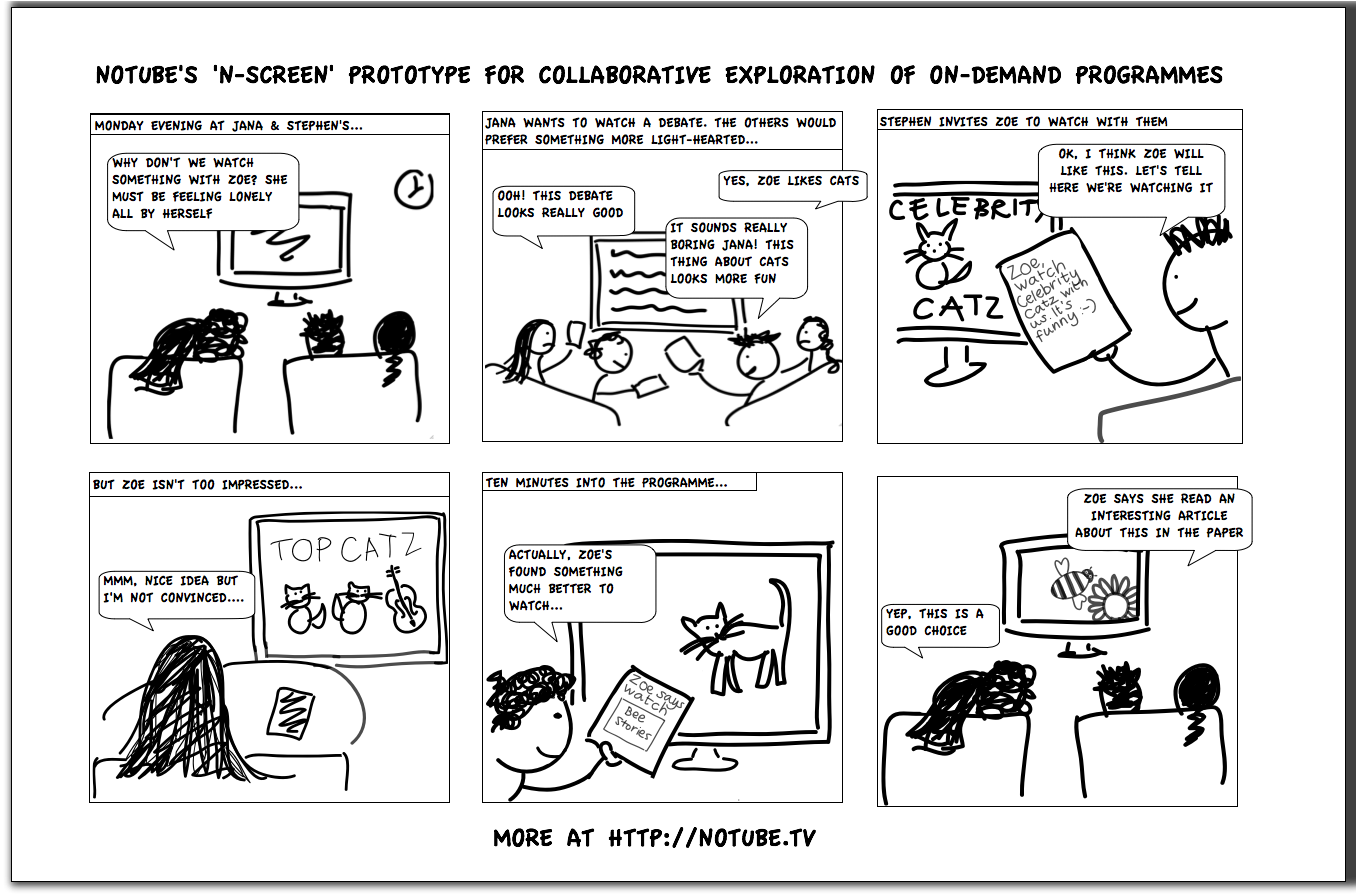
\includegraphics[width=6in]{images/postcard.png}
\caption{A sample NoTube Postcard showing a user scenario} \label{fig:postcard}
\end{center}
\end{figure} 


\section{What have we built?}

We have made prototypes in three main areas:

\begin{itemize}
\item{Live TV Companion}
\item{On-demand browsing}
\item{Authoring second screen content}
\end{itemize}

\section{Live TV Companion}

\subsection{iPhone Remote}

Our first prototype was a second screen iPhone application that worked with MythTV, an open source software TV receiver, to display information related to the programme. Instead of being specifically designed for that particular piece of software, we designed an API (`Buttons') to generalise over multiple devices and applications. The underlying backend was XMPP (Extensible Messaging and Presence Protocol), an XML messaging framework with identity, contact and group management. 

\begin{figure}[htbp]
\begin{center}
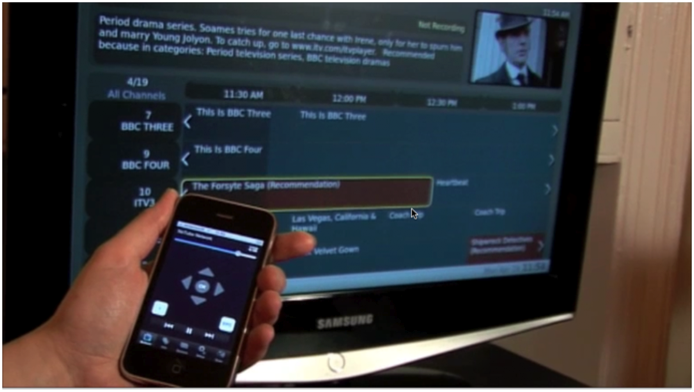
\includegraphics[width=6in]{images/year1.png}
\caption{iPhone remote in action} \label{fig:year1}
\end{center}
\end{figure} 

From this prototype we learned several things:

\begin{itemize}
\item{IPhone prototyping is comparatively slow}
\item{It is difficult to automate finding content related to a particular programme, and although identification of a programme takes place in the production of metadata, this identification is not made available in a useful form to end users}
\item{XMPP is a promising technology for syncing between devices, allowing us to punch through firewalls and host infrastructure on external servers}
\item{A substantial amount of infrastructure was missing to make social TV real beyond the obvious and already-existing techniques (such as having a `Twitter' or `Facebook' button)}
\end{itemize}

In order to be able to create prototypes quickly, after the first year we moved to HTML / Javascript using an XMPP backend infrastructure and APIs over the top of that. We built some of the infrastructure we needed (for example a crid to pid mapper\footnote{\url{http://notube.tv/2010/08/26/connecting-broadcast-tv-and-the-web-using-a-resolver/}}, allowing us to go from over the air identifiers to HTML, linkable, human-readable content) and tried to persuade people in the industry of the importance of URLs for programmes for word-of-mouth communication, metadata as an advert for content, and the usefulness of APIs to TV.\footnote{\url{http://www.w3.org/2010/11/web-and-tv/papers/webtv2_submission_60.pdf}}

Although we did create some prototypes to be used with live TV (for example, `Votey', a application to allow real-time voting and visualisation of votes for a particular programme \footnote{\url{http://jabber.notu.be/thekilling/}}), and an autocompleting twitter API for TV\footnote{\url{http://notube.tv/2010/11/22/epg-autocompleter/}} most effort after this period has been spent on considering the various problems of on-demand content, particularly the problem of collective choice within large corpuses of content.

\begin{figure}[htbp]
\begin{center}
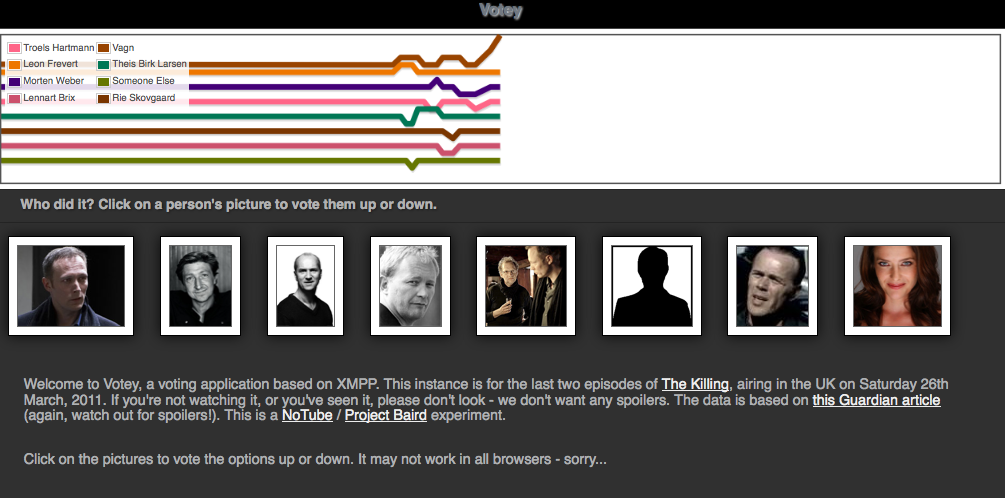
\includegraphics[width=6in]{images/votey.png}
\caption{`Votey' - Real-time graphing of votes} \label{fig:votey}
\end{center}
\end{figure} 

\section{On-Demand Prototypes}

We have made two main prototypes in the on-demand area, both centred around problems of choice.

\subsection{Archive Browser}

This is an HTML-based browser of a subset of BBC's Redux project\footnote{\url{http://www.bbc.co.uk/blogs/bbcinternet/2008/10/history_of_the_bbc_redux_proje.html}} designed to test experimentally if people spent more time browsing and adding to a playlist if related content was presented to them\footnote{\url{http://notube.tv/2011/07/01/finding-interesting-new-programmes-trial-results/}}. We did a randomised trial using 90 volunteers from within the BBC. The results were inconclusive, although people liked the approach whichever group they were placed in -  but one interesting thing did emerge: people like having a `random' (or `shuffle') button. We also made the data for this experiment open for others to download and use. \footnote{\url{http://notube.tv/2011/02/15/linking-wikipedia-and-bbc-programmes/}}.

\begin{figure}[htbp]
\begin{center}
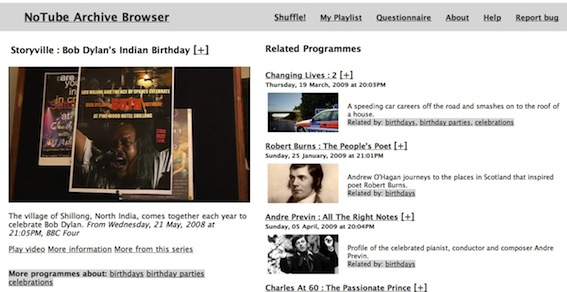
\includegraphics[width=6in]{images/notube-archive-browser.jpg}
\caption{NoTube Archive Browser} \label{fig:archive}
\end{center}
\end{figure} 


\subsection{`N-Screen'}

N-Screen explicitly addresses issues of choice in a social situation. Because people have preferences about each others' mental states (i.e. whether they will also enjoy a programme), choosing in small groups can be very difficult. 

N-Screen is a second screen HTML / Javascript application that allows people to express their preferences to each other directly, by dragging and dropping content to each other individually or as a group. Group members can be in the same room or physically distant, and one or more TVs can be synced to watch together remotely. It is primarily for tablets and laptops, but runs on anything with a modern Web browser; from smartphones to touch-tables and desktop PCs. It is designed for multiple screens in use while watching TV, explicitly addressing the `second screen' issues (but taking it a logical step further), but also some of the social aspects of TV watching, ones that we believe have not been addressed elsewhere.

We have made three different version of N-Screen with three different sets of content: Redux, TED Talks, and iPlayer\footnote{\url{http://notube.tv/2011/10/10/n-screen-a-second-screen-application-for-small-group-exploration-of-on-demand-content/}}, with different approaches to content to content recommendation encapsulated within each, depending on the data available\footnote{\url{http://notube.tv/2011/10/14/algorithms-for-recommendations-in-various-n-screen-implementations/}}.

We are indebted to the VU for their work in arranging for design help, and to Fabrique\footnote{\url{http://www.fabrique.nl/}} for designs to improve the appearance of N-Screen.

\begin{figure}[htbp]
\begin{center}
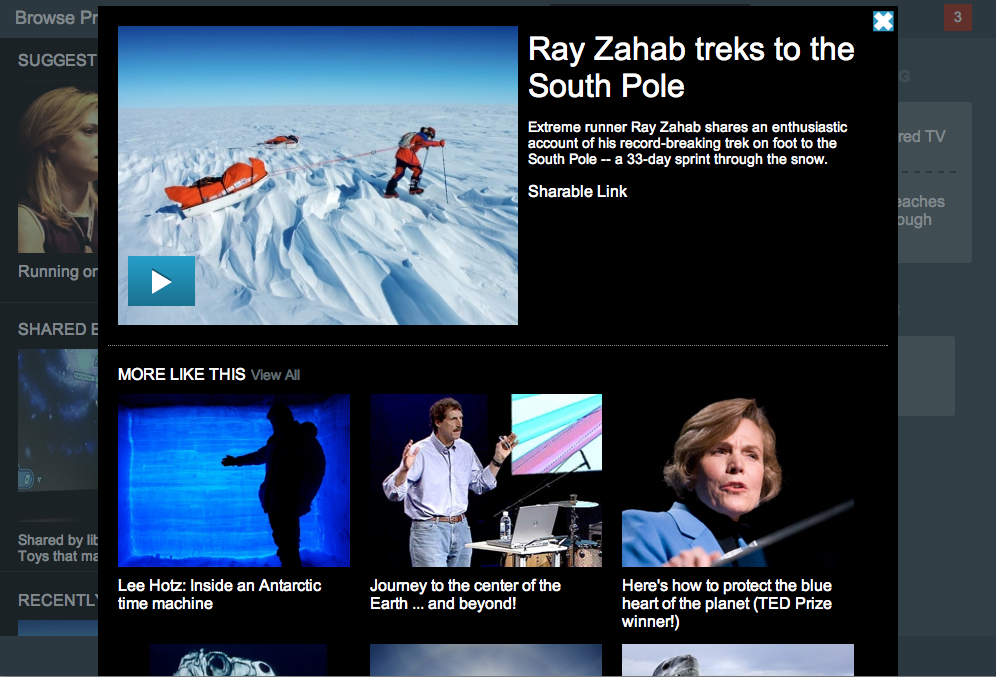
\includegraphics[width=6in]{images/nscreen.png}
\caption{N-Screen - small-group collaborative browsing of video collections} \label{fig:nscreen}
\end{center}
\end{figure} 


\section{Tools for Authoring and Playback of Second Screen Content}

Our final set of demonstrators starts to consider some of the problems with authoring second screen content, and whether collaboration can help. It uses the same infrastructure as N-Screen but shows some of the different ways it can be used.

\subsection{TV Extras Authoring (`TEA')}

TEA lets you author basic extras for the second screen, as you watch a video, using drag and drop from searches of the web. It is a web application built using HTML5. The usecases concern:

\begin{itemize}
\item{Professional, common-place second screen content authoring within organisations}
\item{Enthusiast annotation}
\end{itemize}

Currently we only address on-demand authoring.

In the application, two or more people can see each others' suggestions for second screen links and review it. Either can then sync the video for playback, so they can review it together. Finally, they can save their work to an intermediate file format for playback on other devices. This intermediate file is in some ways the most interesting part, as it enables expert developers for particular platforms to create second screen playback tools without also having to handle the authoring side.

\begin{figure}[htbp]
\begin{center}
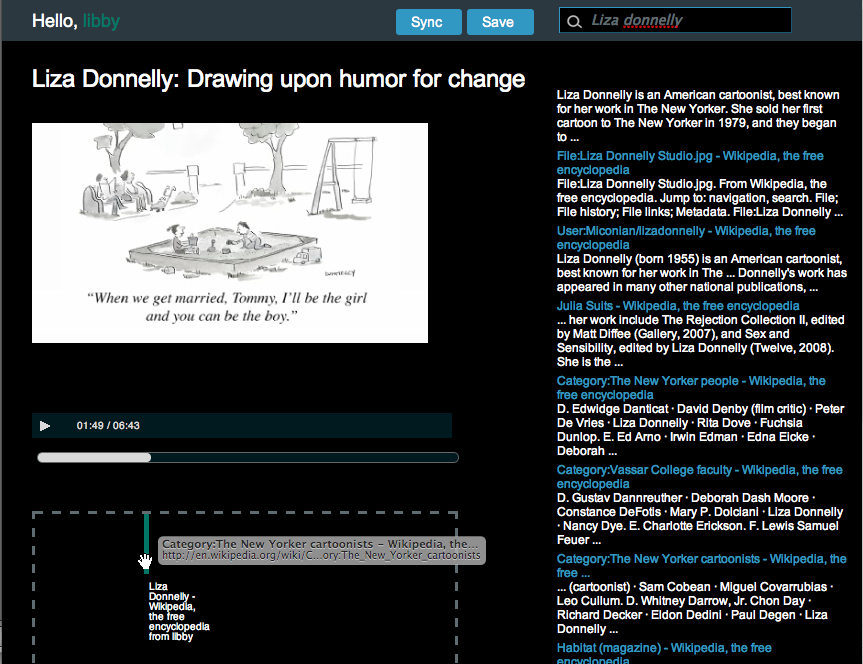
\includegraphics[width=4in]{images/tea.png}
\caption{`TEA' - TV Extras Authoring} \label{fig:tea}
\end{center}
\end{figure} 


\subsection{TEAPlayer}

TEAPlayer is an experimental iPhone application built with Phonegap\footnote{\url{http://www.phonegap.com/}}(so the bulk of it is HTML) to play the output format of TEA on XBMC (XBox Media Centre). The idea was to see if the information in the file format produced using TEA was sufficient to be made into a useful tool. The result is an iPhone application that looks for XBMC (a video player) instances on the same network, and allows the user to choose from a selection of videos on an iPhone to play on it. If she chooses an annotated video, it loads the URLs on the iPhone at the correct time during playback. It also enables her to pause and play the currently playing video.

\begin{figure}[htbp]
\begin{center}
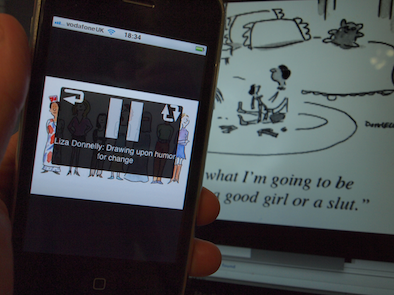
\includegraphics[width=3in]{images/tea_player1.png}
\caption{`TEAPlayer' - Second screen video content player} \label{fig:teaplayer1}
\end{center}
\end{figure} 

\begin{figure}[htbp]
\begin{center}
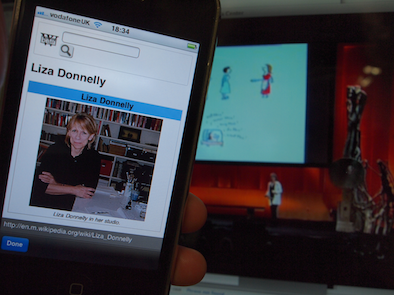
\includegraphics[width=3in]{images/tea_player2.png}
\caption{`TEAPlayer' - Second screen video content player} \label{fig:teaplayer2}
\end{center}
\end{figure} 

\section{What have we learned?}

Our conclusions remain the same as those expressed a year ago in our paper to the Web and TV workshop in Berlin (with Mo McRoberts)\footnote{\url{http://www.w3.org/2010/11/web-and-tv/papers/webtv2_submission_60.pdf} (pdf)}. We enumerated the key problems facing developers of second screen content:

\begin{itemize}
\item{(a) How do we know what the person is watching?}
\item{(b) How do we locate additional information about the programme?}
\item{(c) How do we locate apps or Web pages related to it?}
\item{(d) How can we manipulate it?}
\end{itemize}

We proposed three parts of a solution

\subsection{Use metadata as an advert for the content that can flow out into the public Web in search of viewers}
\subsection{Create URLs for the content items}
\subsection{Agree on open APIs for controlling the TV and getting access to metadata from it}

The only thing we would add to that at this stage is that we failed to completely understand and emphasise the huge gap between web developers and TV developers. To harness the creativity of the vast number of web developers, a TV API needs to be extremely easy to use and understandable within a page or two of documentation. This is a very, very different way of working to TV developers, and there is a large chasm of understanding between the two groups.

It was very disappointing to see a plethora of `Apps' and APIs to TV at IBC 2011, with no standard in place to mitigate the effect of this diversity on consumers and developers.

\section{Next steps}

In the final three months of the project we want to tackle the following final tasks:

\subsection{Integration of personalised recommendations}

N-Screen provides the capacity for several different kind of recommendations, including personalised ones from a source such as Beancounter. We are mid-way though a lightweight integration of Beancounter and N-Screen, using Beancounter as a datasource for N-Screen and vice-versa.

\subsection{Evaluation and user testing}

Two pieces of user testing are planned:

\begin{itemize}
\item{General comparison of second screen and on-screen information}
\item{User evaluation of N-Screen}
\end{itemize}

\subsection{Refining the TEA file format}

We are researching possible existing formats for describing URL-based annotation at points in a video.

\subsection{Completing and publishing an implementation of the `Buttons' Javascript API}

This will allow developers to use second screen applications without worrying about the detail of the XMPP infrastructure.


\end{document}


%\begin{figure}[htbp]
%\begin{center}
%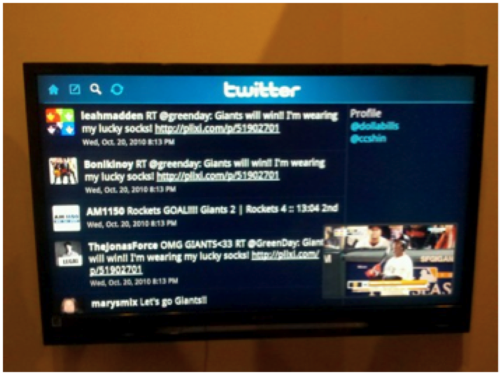
\includegraphics[width=6in]{images/googletv.png}
%\caption{Twitter on GoogleTV} \label{fig:google}
%\end{center}
%\end{figure} 
